\documentclass[a4paper,11pt]{article}
\usepackage{configuration}


\begin{document}
%\begin{titlepage}
 \thispagestyle{empty}
\begin{center}
 
\textsc{\LARGE Université de Mons-Hainaut}\\[0.5cm]
\textsc{\Large Faculté des Sciences}\\[4.0cm]
\textsc{\Large Simulation de systèmes à évènements discrets}\\[0.5cm]
 
 
% titre
\HRule \\[0.4cm]
{ \Large \bfseries Rapport du projet}\\[0.3cm]
 
\HRule \\[1.5cm]
 
% auteur et directeur
\begin{minipage}{0.4\textwidth}
\begin{flushleft} \large
\emph{Auteurs:} 
\\ Sébastien \textsc{Dubois}
\\ Jean-François \textsc{Mernier}
\\ Frédéric \textsc{Regnier}

\end{flushleft}
\end{minipage}
\begin{minipage}{0.4\textwidth}
\begin{flushright} \large
%\emph{Directeur:} \\ Olivier \textsc{Markowitch}
\end{flushright}
\end{minipage}


% remplit la page (de vide :p)
\vfill

% date avec un peu d'espace ensuite
{\Large \today}\\[1.5cm]

% logos en bas de page

\includegraphics[scale=0.03]{umh/logo-acwalbxl.png}

\includegraphics[scale=0.08]{umh/logo-umh.png}

\end{center}


% ajoute une page vierge après la page de garde
\newpage
\thispagestyle{empty}
\mbox{}
\newpage
%\end{titlepage}

\tableofcontents % table des matières
%\pagebreak
\listoffigures % liste des figures
%\pagebreak
\lstlistoflistings
\pagebreak
%\listoftables % liste des tables
%\pagebreak




\section{Décisions}

\subsection{Gestion des évènements}
Nous avons choisi d'utiliser une seule FEL pour la simulation. On y place tous les évènements. De plus, pour un temps $t$ de simulation donné, nous avons décidé de traiter certains évènements prioritairement:

\begin{enumerate}
 \item En premier lieu on traite les évènements de réception d'informations de routage
 \item Puis les évènements de réception d'informations de routage
 \item Puis les évènements de réception de messages (accusés et messages normaux)
 \item Puis les évènements de timeout (un message pour lequel on a pas encore reçu d'accusé)
\end{enumerate}

Une fois tous ces évènements traités pour un temps $t$, on traite les autres selon l'ordre \textit{FIFO}.

\subsection{Distance vector}
Nous avons choisi de modifier les coûts en fonction du taux d'occupation du buffer de l'agent. Ceci est expliqué à la section \refp{evt-agent-reception-message} concernant l'évènement de réception d'un message par un agent.

Nous avons aussi implémenté la technique du \textit{poisonned reverse} comme expliqué dans l'article concernant le distance vector.








\section{Evenements}

\begin{figure}[h!t]
  \centering
    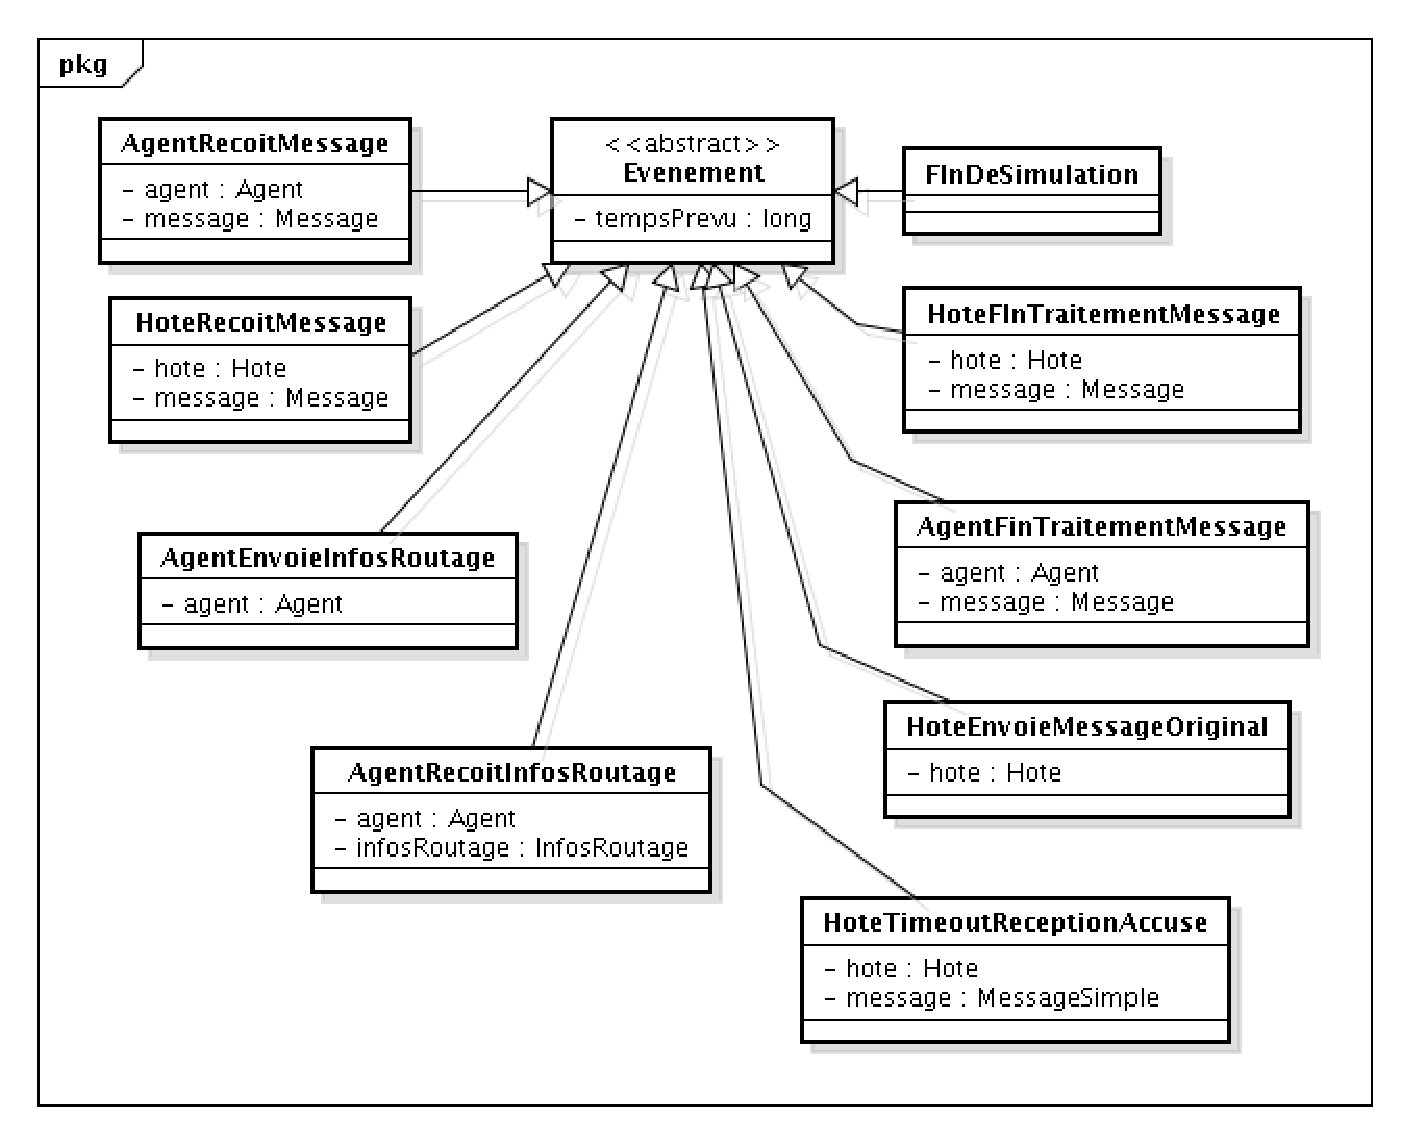
\includegraphics[scale=0.60]{Evenements}
  \caption{Evènements}
  \label{fig:evenements}
\end{figure}




\subsection{Hotes}


\subsubsection{Envoi d'un message original}
L'envoi d'un message original par un hôte est illustré par la figure \refp{fig:hote-envoie-message-original}. 

\begin{figure}[h!t]
  \centering
    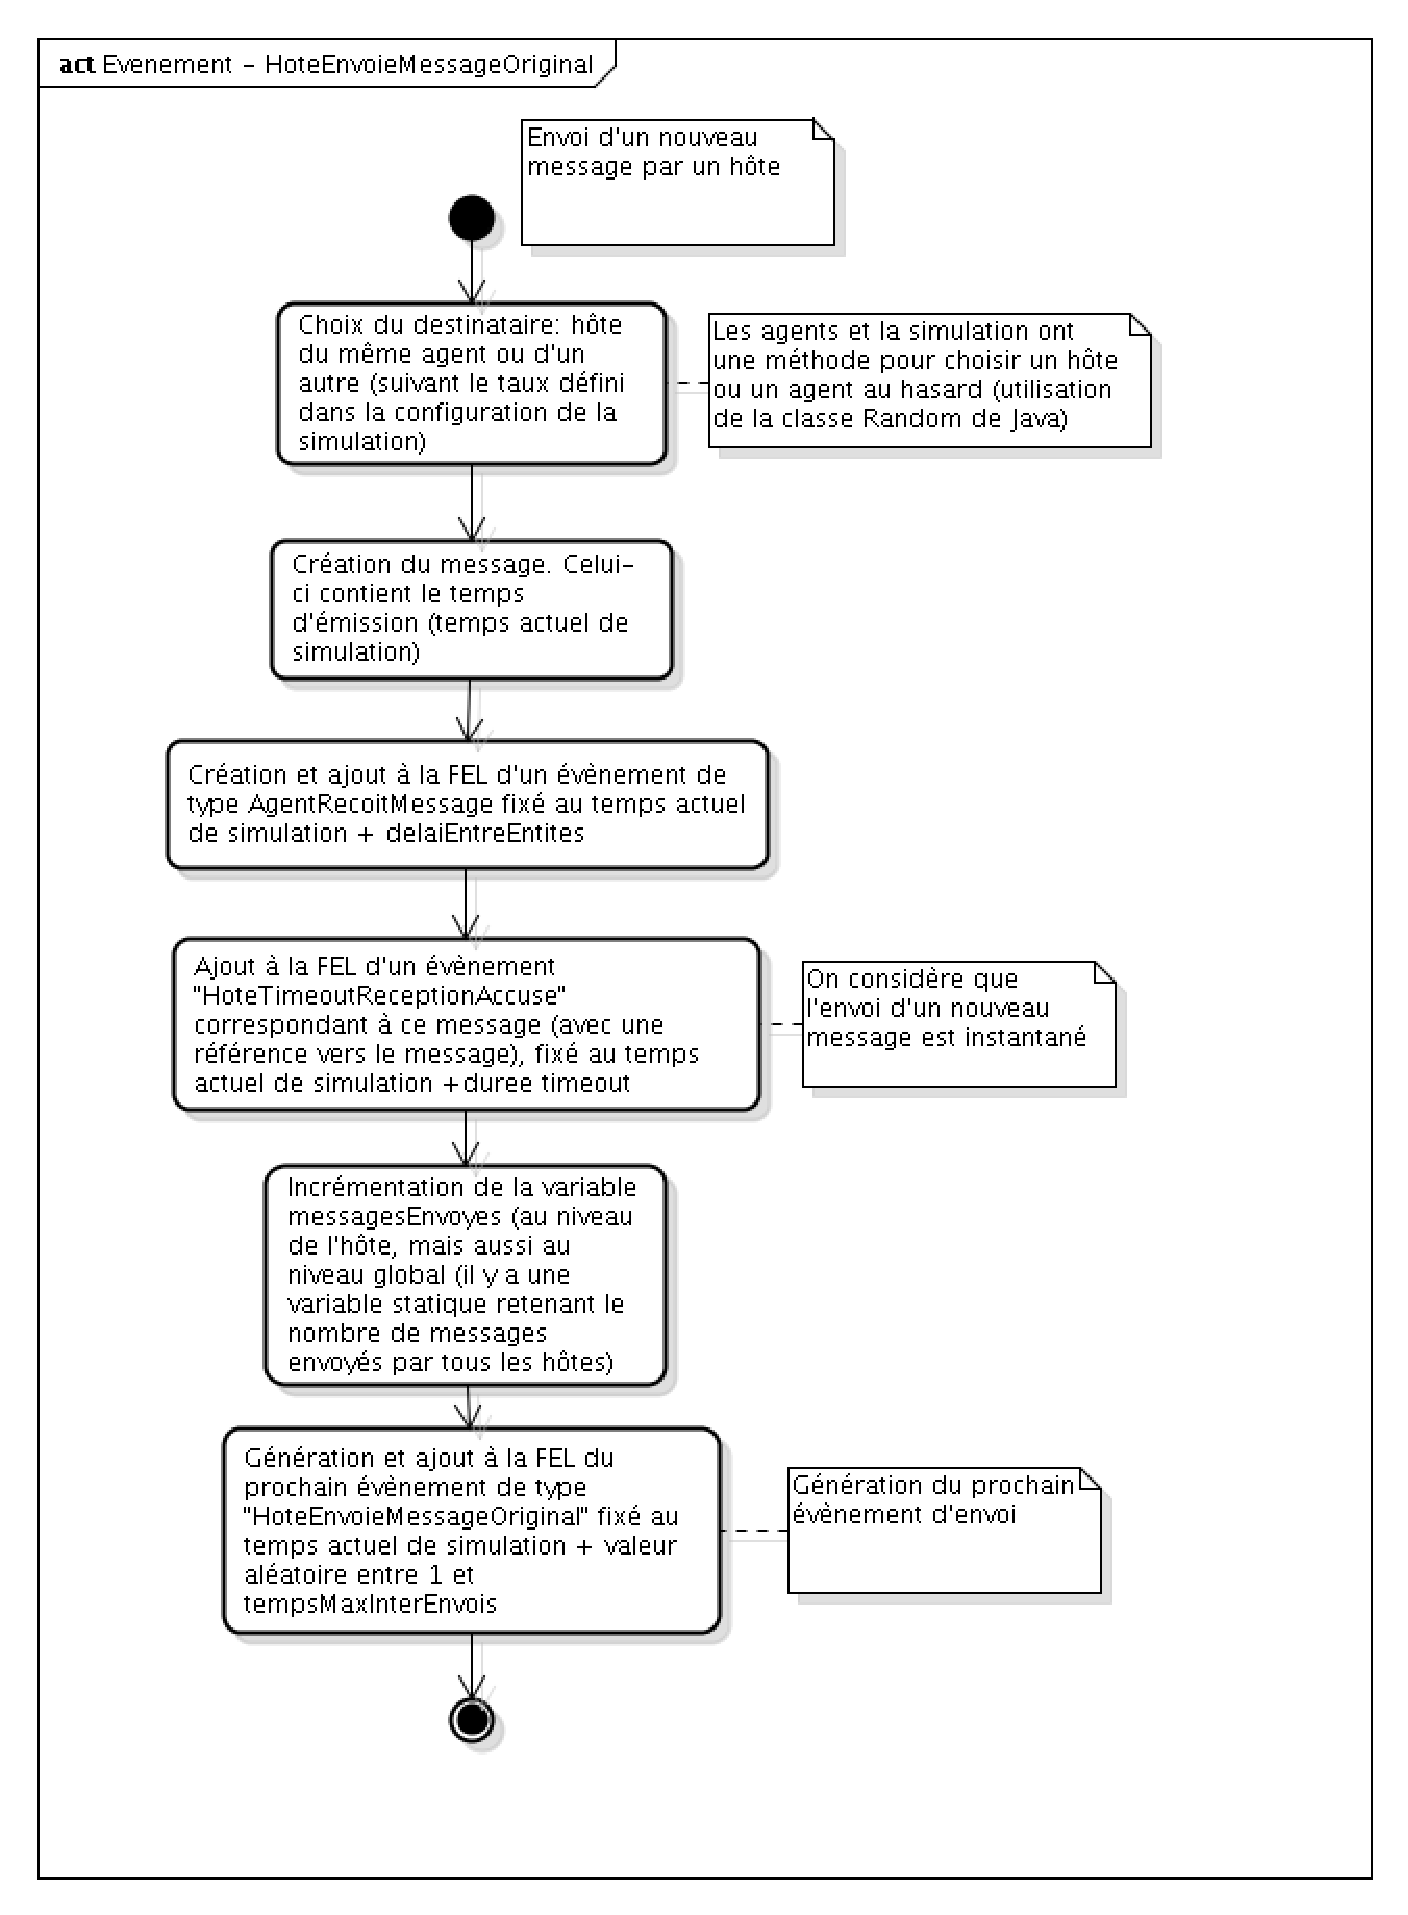
\includegraphics[scale=0.60]{HoteEnvoieMessageOriginal}
  \caption{Envoi d'un message original par un hôte}
  \label{fig:hote-envoie-message-original}
\end{figure}

Comme le diagramme le montre, nous avons choisi de ne générer qu'un évènement d'envoi à la fois. Nous générons et plaçons le premier évènement sur la FEL. Quand celui-ci devient l'évènement imminent, l'hôte crée et envoie son message et génère l'évènement suivant puis le place sur la FEL.


\clearpage
\subsubsection*{Génération des temps d'envoi}
Une variable aléatoire nous permet de générer pour chaque hôte le temps du prochain envoi (entre le temps actuel de simulation + 1 et le temps actuel de simulation + le temps inter-envois). Pour ce faire, chaque hôte dispose de sa propre instance:

\begin{lstlisting}[caption=Génération des temps d'envoi]
private final Random generateurTempsEnvoi = new Random();

...

/**
 * Generer le prochain temps d'envoi.
 *
 * @return le prochain temps d'envoi.
*/
private long genererTempsProchainEnvoi() {
	int tempsAvantProchainEnvoi =
			generateurTempsEnvoi.nextInt(getConfiguration()
					.getConfigurationHotes().getTempsMaxInterEnvois()) + 1;
	// on fait +1 et donc par exemple 0-5 devient 1-6
	return getSimulation().getHorloge() + tempsAvantProchainEnvoi;
}
\end{lstlisting}





\subsubsection*{Choix du destinataire}
Un paramètre de simulation permet de spécifier le pourcentage de messages qui doivent être à destination d'un hôte connecté à un autre agent. Pour implémenter ceci, nous avons utilisé deux autres variables aléatoires. Chaque hôte dispose d'une variable aléatoire qu'on utilise avec des random digits de la manière suivante:

\begin{lstlisting}[caption=Choix du type de destinataire d'un message]
private final Random generateurTypeDestination = new Random();

...

int randomDigitsAutreAgent =
	(int) (getConfiguration().getConfigurationHotes()
	.getTauxMessagesVersAutreAgent() * 100);
int random = generateurTypeDestination.nextInt(100) + 1;
boolean messagePourHoteAutreAgent = false;

if (random <= randomDigitsAutreAgent) {
	messagePourHoteAutreAgent = true;
}
\end{lstlisting}










\clearpage

D'un autre côté, des méthodes se servant de variables aléatoires permettent de choisir un agent ou un hôte aléatoirement. De cette façon, un hôte peut déterminer de manière aléatoire qui devra reçevoir son message:

\begin{lstlisting}[caption=Hote - Choix de la destination]
if (messagePourHoteAutreAgent) {
	hoteDestination = getSimulation().getAgentAleatoire(this.getAgent()).getHoteAleatoire();
}
else {
	hoteDestination = this.getAgent().getHoteAleatoire(this);
}
\end{lstlisting}




\clearpage

Dans le premier cas, si le message doit être à destination d'un hôte connecté à un autre agent, l'hôte demande un agent aléatoire avec comme exception son propre agent (puisque ça doit être n'importe quel agent autre que le sien). Dans le second, l'hôte demande simplement à son agent de choisir un de ses hôtes aléatoirement (à l'exception de l'hôte actuel). Par exemple, voici la méthode permettant d'obtenir un agent aléatoire:

\begin{lstlisting}[caption=Utilisation des variables aléatoires pour sélectionner un agent]
/**
 * PRNG utilise pour choisir un agent au hasard.
*/
private final Random		generateurChoixAgent	= new Random();
	
...

/**
 * Recuperer un agent aleatoire pouvant etre n'importe lequel sauf celui
 * fourni en argument.
 * 
 * @param exception
 *        le seul agent ne pouvant pas etre retourne
 * @return un agent aleatoire autre que celui donne en argument
*/
public Agent getAgentAleatoire(final Agent exception) {
	Agent retVal = null;
	do {
		switch (generateurChoixAgent.nextInt(7) + 1) {
			case 1:
				retVal = agent1;
				break;
			case 2:
				retVal = agent2;
				break;
			case 3:
				retVal = agent3;
				break;
			case 4:
				retVal = agent4;
				break;
			case 5:
				retVal = agent5;
				break;
			case 6:
				retVal = agent6;
				break;
			case 7:
				retVal = agent7;
				break;
			default:
				LOGGER
						.error("Un probleme a eu lieu pendant la selection aleatoire d'un agent.");
		}
	} while (retVal == null || exception.equals(retVal));
	
	return retVal;
}
\end{lstlisting}

\clearpage











\subsubsection{Réception d'un message}
La réception d'un message par un hôte est illustrée par la figure \refp{fig:hote-recoit-message}.

\begin{figure}[h!t]
  \centering
    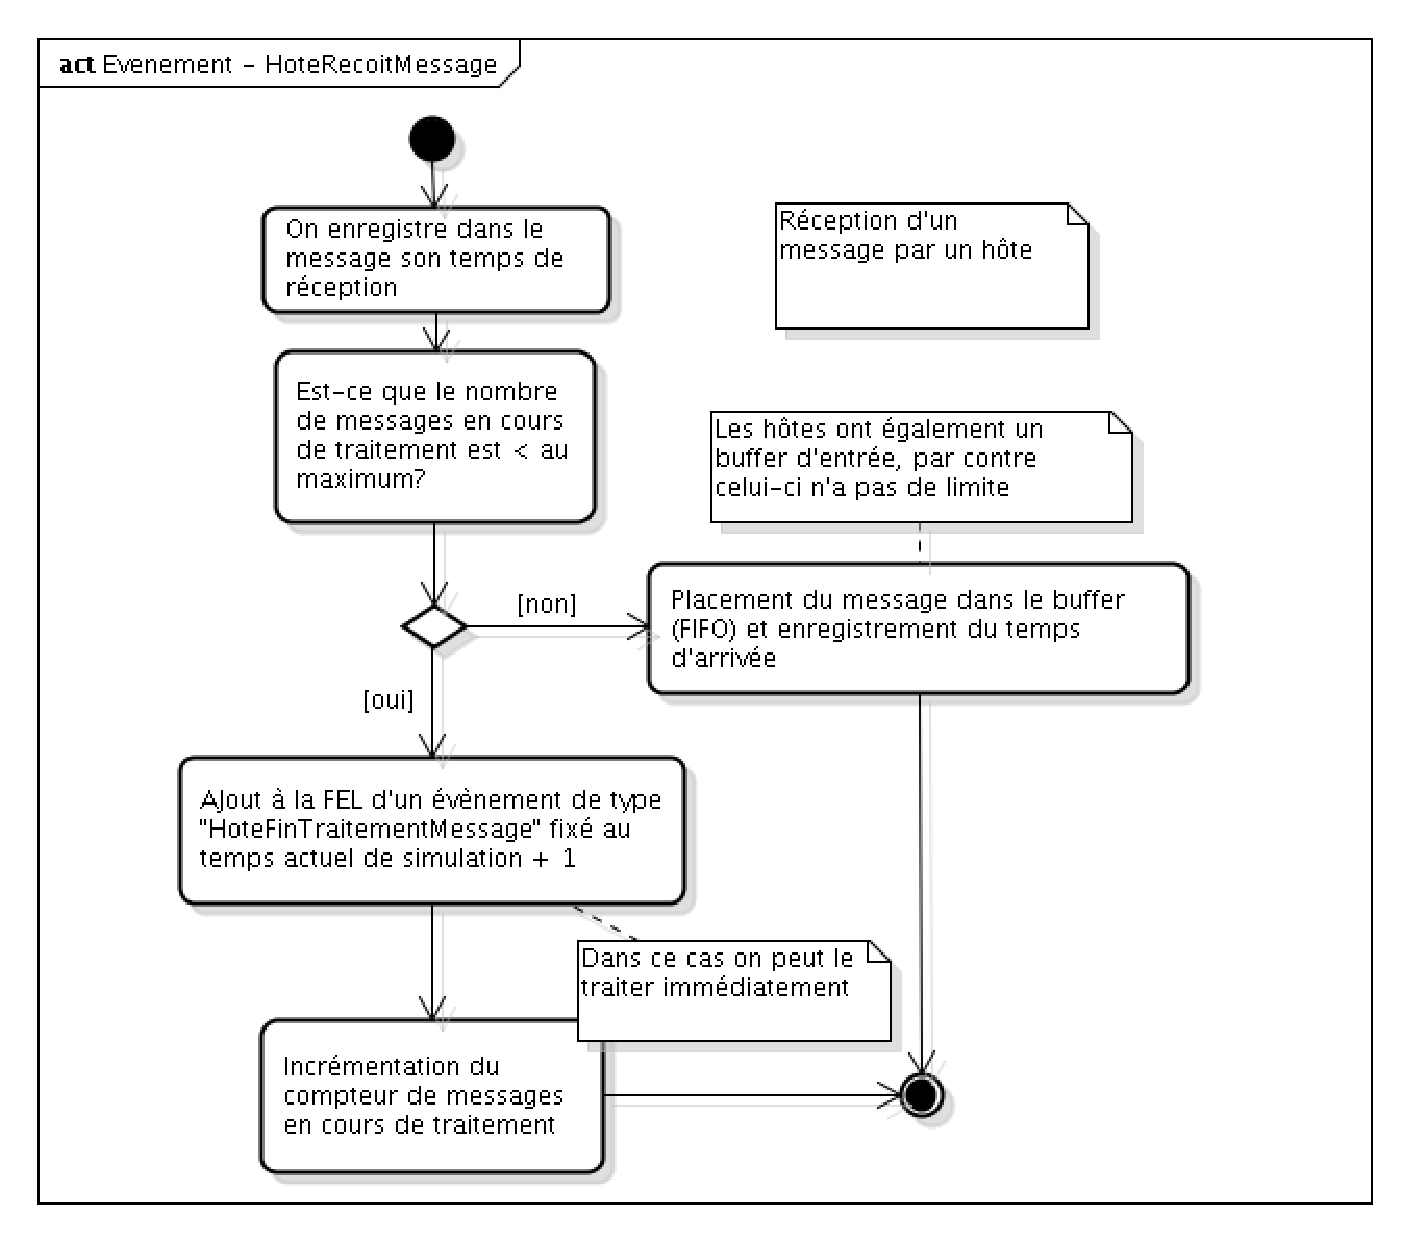
\includegraphics[scale=0.60]{HoteRecoitMessage}
  \caption{Réception d'un message par un hôte}
  \label{fig:hote-recoit-message}
\end{figure}








\subsubsection{Fin de traitement d'un message}
Le diagramme UML correspondant étant trop grand, nous ne l'avons pas inclus dans le rapport. Il est disponible dans le dossier \textbf{UML} qui accompagne le rapport (le fichier: \textbf{Evenement - HoteFinTraitementMessage.png}).




\subsubsection{Timeout}
Les actions prises lors d'un timeout sont illustrées par la figure \refp{fig:hote-timeout}.

\begin{figure}[h!t]
  \centering
    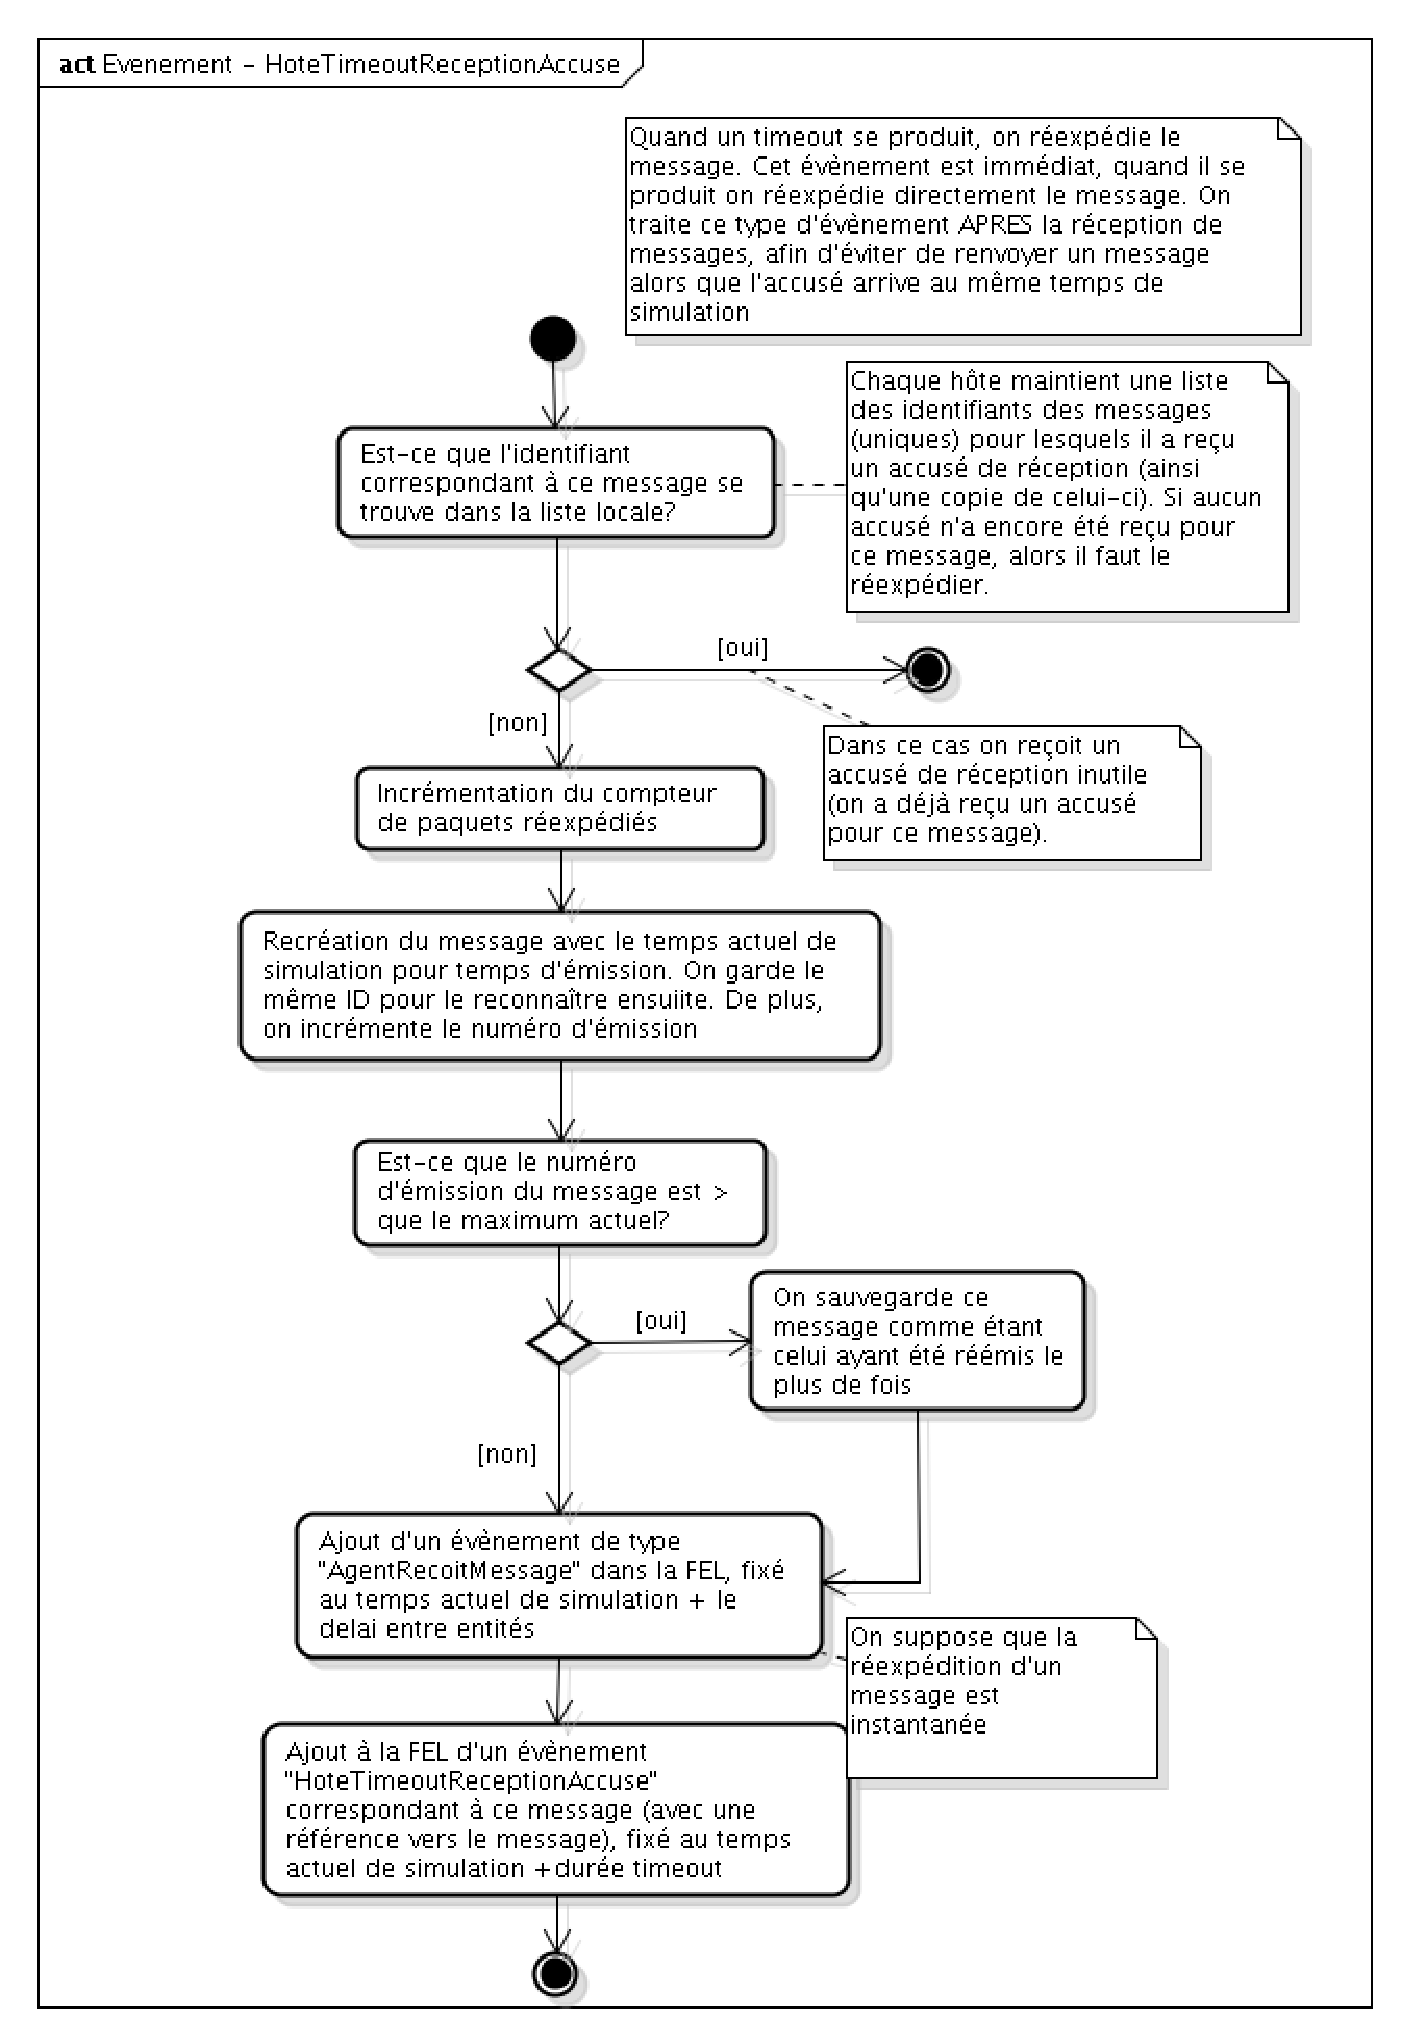
\includegraphics[scale=0.60]{HoteTimeoutReceptionAccuse}
  \caption{Timeout de réception d'un accusé}
  \label{fig:hote-timeout}
\end{figure}











\subsection{Agents}


\subsubsection{Réception d'un message}\label{evt-agent-reception-message}
Le diagramme UML correspondant étant trop grand, nous ne l'avons pas inclus dans le rapport. Il est disponible dans le dossier \textbf{UML} qui accompagne le rapport (le fichier: \textbf{Evenement - AgentRecoitMessage.png}).

Dans le diagramme UML, il y a deux points que nous n'avons pas expliqués (en jaune):

\begin{itemize}
 \item Le premier point: \og Est-ce qu'on peut envoyer les nouvelles informations de routage maintenant? \fg. Nous avons décidé d'éviter trop d'envois successifs inutiles d'informations de routage, afin de ne pas surcharger le système. Pour ce faire, quand un agent doit envoyer les informations de routage (à cause du niveau d'occupation du buffer), il vérifie si ça fait au moins $x$ temps de simulation qu'il a envoyé un message de ce type. Si oui, alors il peut envoyer le message. De cette manière, si pour un temps $t$ donné, l'agent reçoit $50$ messages, que pour le premier il dépasse le seuil d'alerte d'occupation du buffer et envoie ses informations de routage, puisqu'il sera toujours au delà du seuil d'alerte pour les $49$ autres messages, il ne renverra plus de message avant un certain délai.
 
 \item Le second point: \og Augmentation du coût de nos routes à destination des autres agents (on augmente d'une valeur fixe à chaque fois) \fg. Nous faisons ceci afin que le distance vector prenne en compte le niveau d'occupation des buffers des agents. Quand un agent donné est surchargé, il augmente le coût de ses routes à destination des autres agents et prévient ses voisins (i.e., leur envoie son DV). De cette manière quand les voisins reçoivent les informations, ils mettent à jour leur propre table de routage et choisissent peut être d'autres routes pour faire suivre les messages (i.e., changent leur DV). Si les autres agents deviennent surchargés, leurs coûts augmenteront également. Ainsi au final, le DV prend en compte l'occupation des buffers des agents, ce qui permet de mieux répartir la charge sur les différents agents. Dans les résultats des simulations, nous avons en effet constaté que les buffers sont utilisés de manière plus homogène quand le distance vector est activé.
\end{itemize}





\subsubsection{Fin de traitement d'un message}
Le diagramme UML correspondant étant trop grand, nous ne l'avons pas inclus dans le rapport. Il est disponible dans le dossier \textbf{UML} qui accompagne le rapport (le fichier: \textbf{Evenement - AgentFinTraitementMessage.png}).







\subsubsection{Envoi des informations de routage}
L'envoi d'informations de routage (envoi du DV d'un agent à ses voisins) est illustré par la figure \refp{fig:agent-envoi-infos-routage}.

\begin{figure}[h!t]
  \centering
    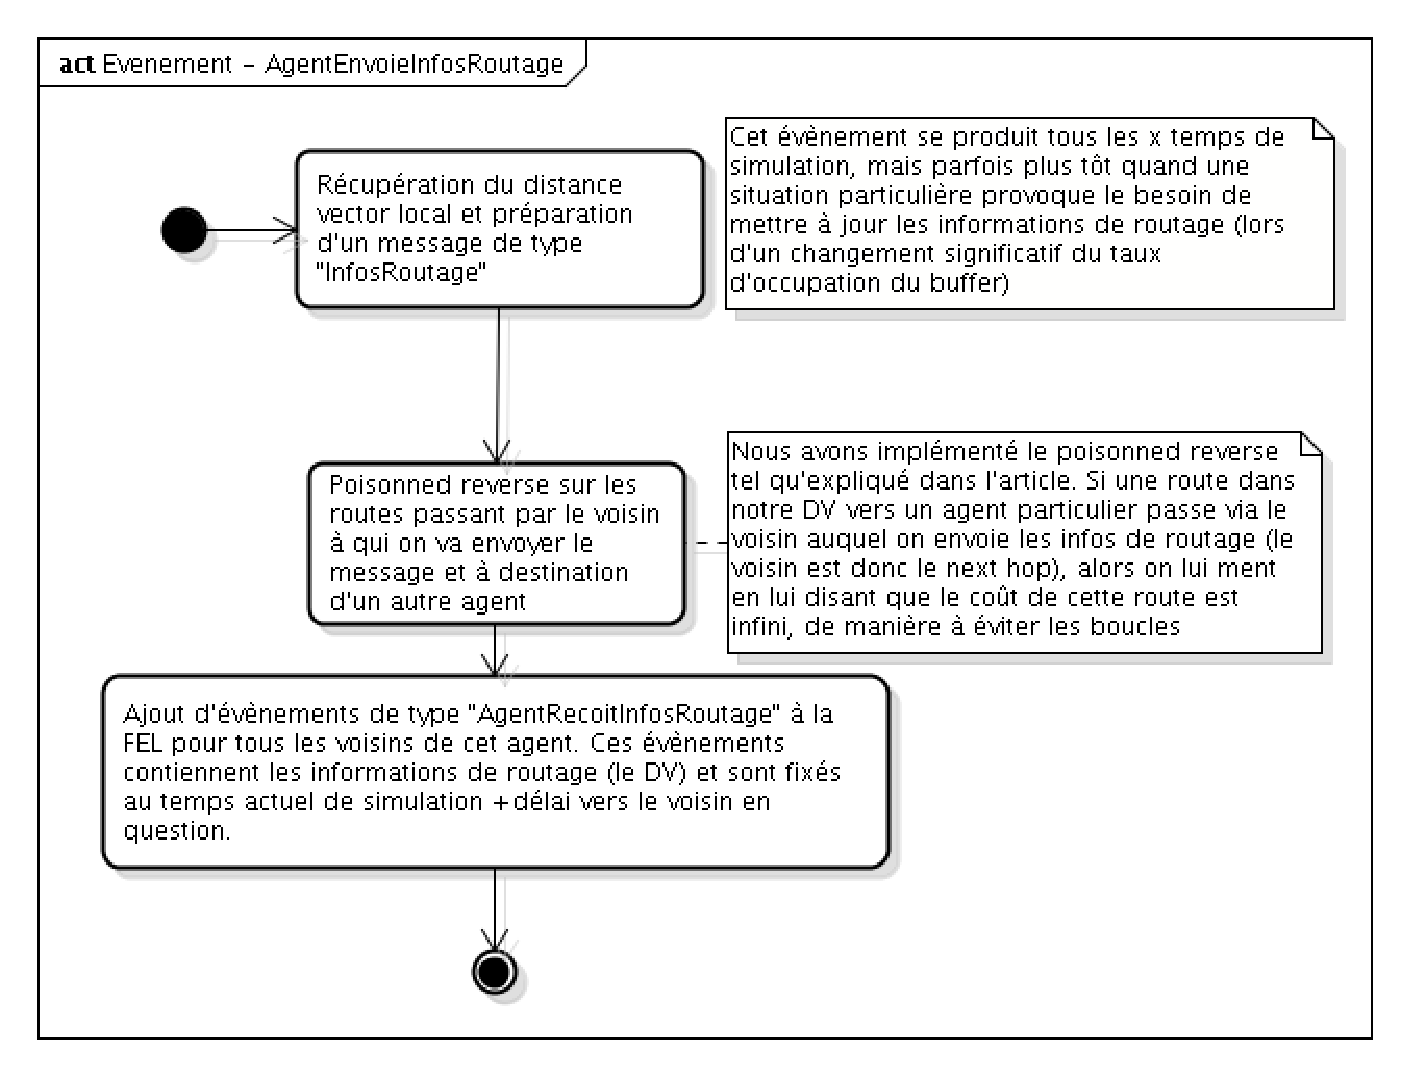
\includegraphics[scale=0.60]{AgentEnvoieInfosRoutage}
  \caption{Envoi d'informations de routage par un agent}
  \label{fig:agent-envoi-infos-routage}
\end{figure}





\subsubsection{Réception d'informations de routage}
La réception d'informations de routage (réception du DV d'un voisin par un agent) est illustrée par la figure \refp{fig:agent-recoit-infos-routage}.

\begin{figure}[h!t]
  \centering
    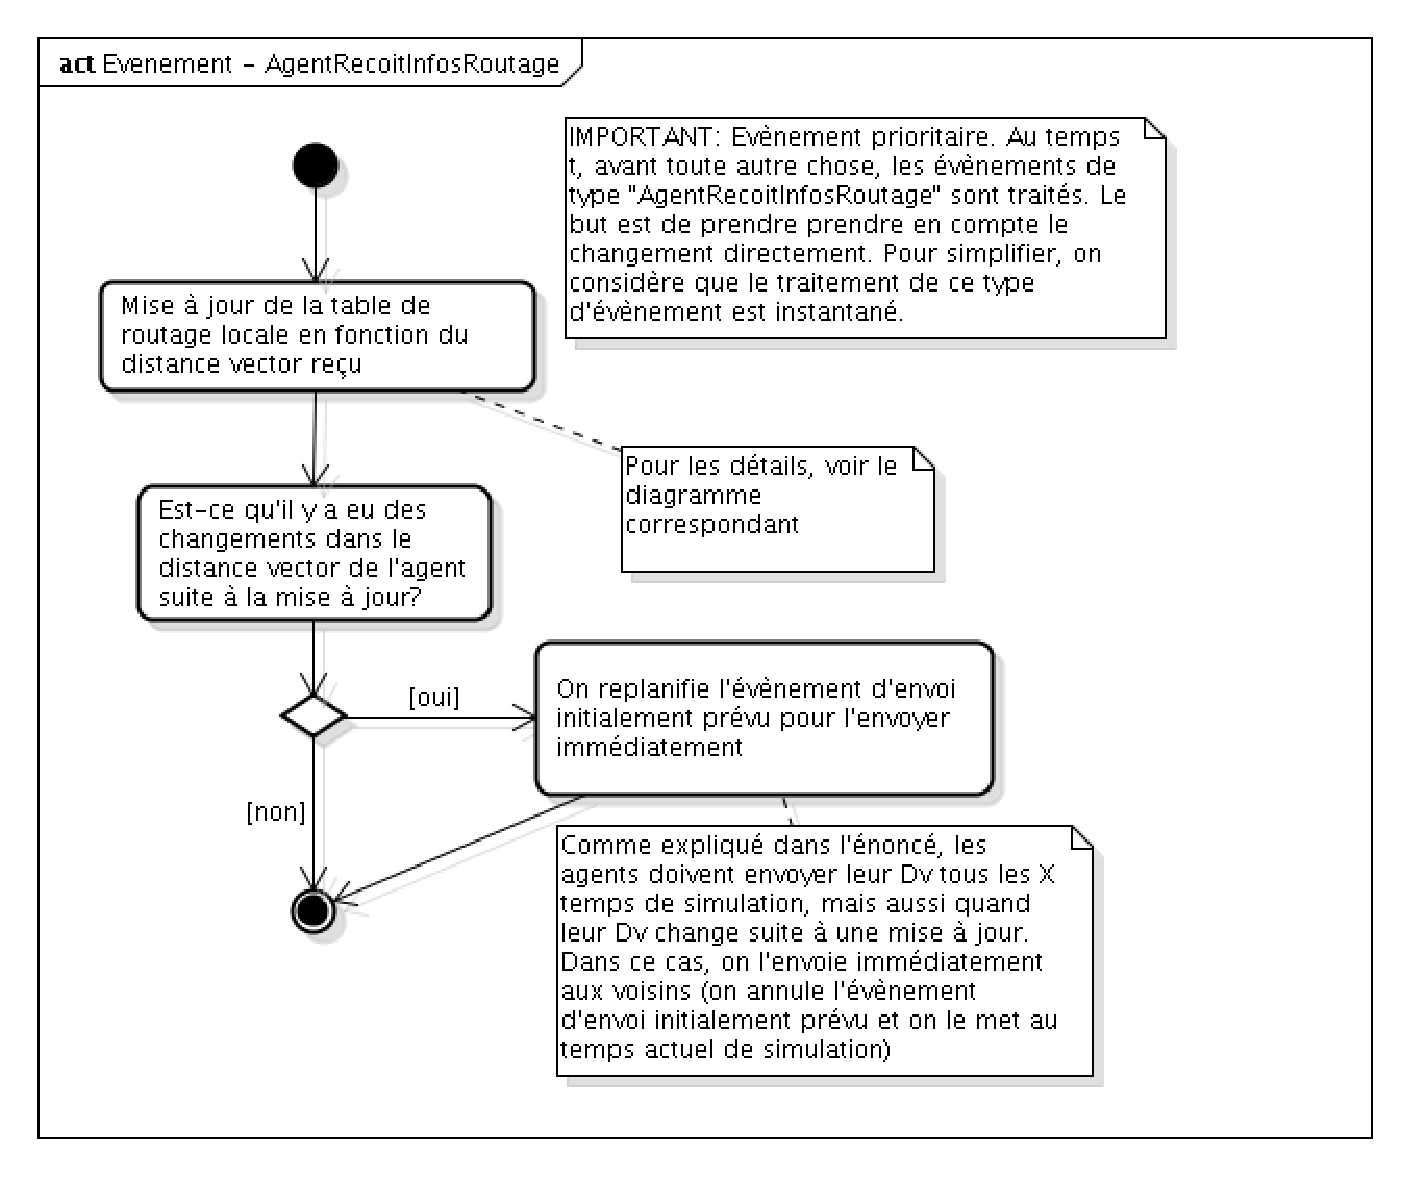
\includegraphics[scale=0.60]{AgentRecoitInfosRoutage}
  \caption{Réception d'informations de routage par un agent}
  \label{fig:agent-recoit-infos-routage}
\end{figure}

Le détail des opérations effectuée lors de la mise à jour (vérifications, etc) n'est pas dans le rapport non plus car le diagramme est trop grand. Le fichier est disponible dans le dossier \textbf{UML} qui accompagne le rapport (le fichier: \textbf{Mise à jour des informations de routage.png}).













\subsection{Autres}

\subsubsection{Fin de simulation}
Le dernier évènement est spécial; c'est celui qui provoque la fin de la simulation. Quand cet évènement devient l'évènement imminent, il remet la FEL à zéro (il n'y a donc plus d'évènement imminent après lui) et la boucle de simulation s'arrête. Le détail est illustré par la figure \refp{fig:fin-de-simulation}.


\begin{figure}[h!t]
  \centering
    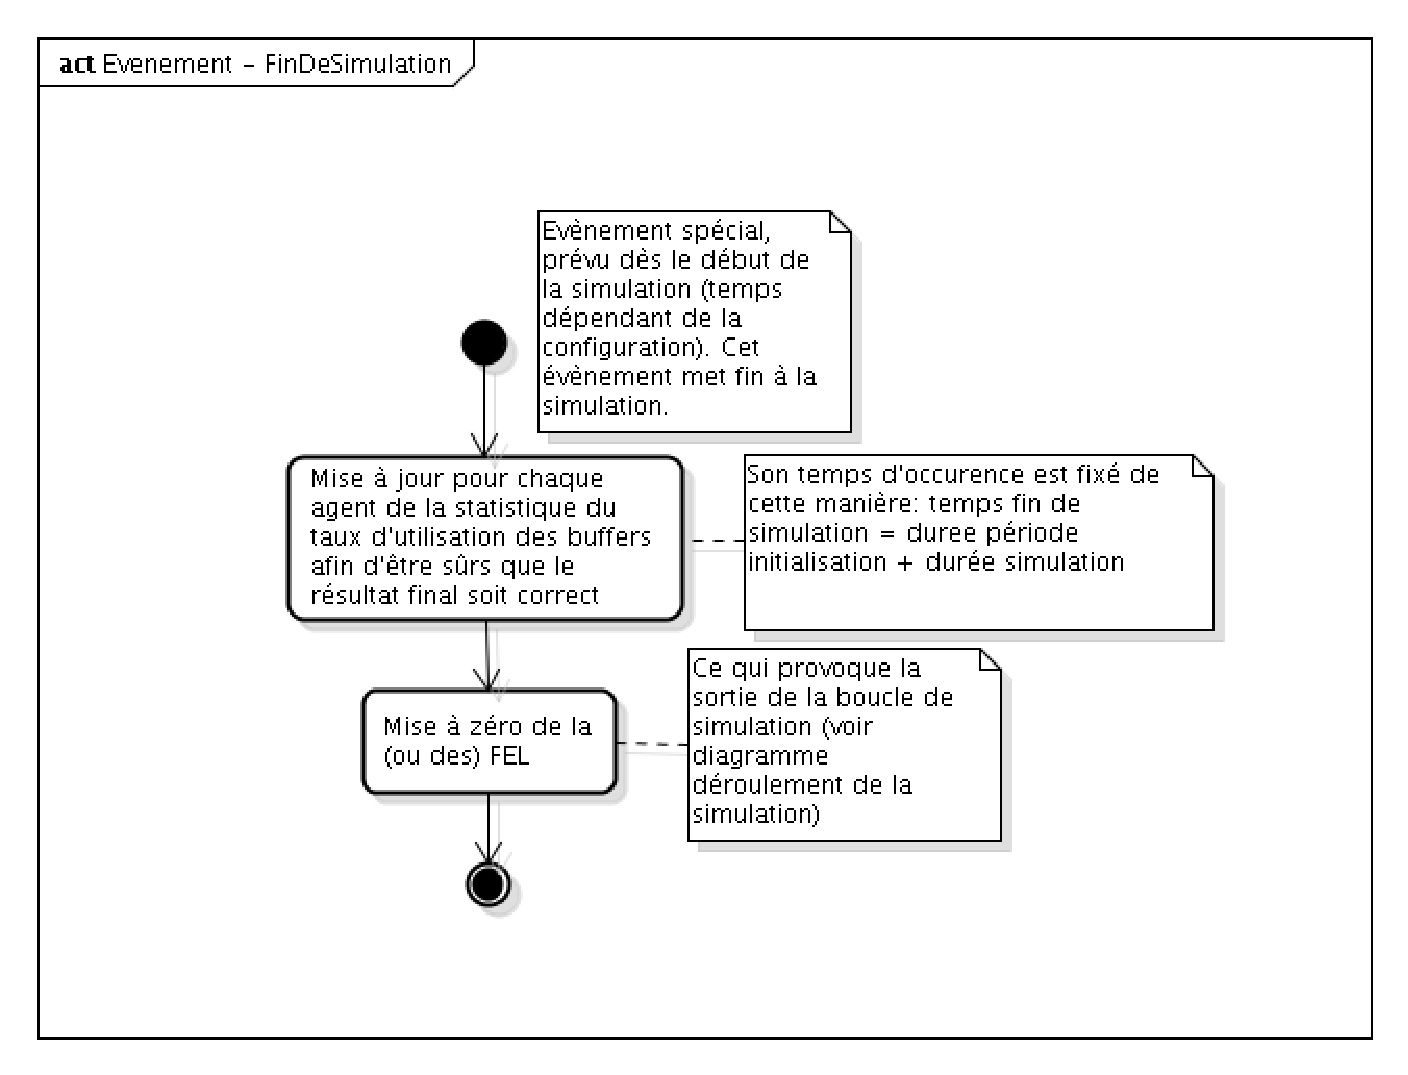
\includegraphics[scale=0.60]{FinDeSimulation}
  \caption{Fin de la simulation}
  \label{fig:fin-de-simulation}
\end{figure}

















\section{Messages}
Les entités de la simulation s'envoient différents types de messages. Un diagramme UML les illustrant existe mais n'a pas été inclus au rapport car il est trop grand. Il est disponible dans le dossier \textbf{UML} qui accompagne le rapport (le fichier: \textbf{CD Messages.png}).








\section{Paramètres du système}

\subsection{Hote}
\begin{itemize}
 \item Durée du timeout (temps après lequel on réémet un message)
 \item Temps maximal inter-envois (pour les messages originaux)
 \item Temps de traitement d'un message
 \item Pourcentage de messages à destination d'un autre agent
\end{itemize}


\subsection{Agent}

\begin{itemize}
 \item Nombre d'hôtes reliés
 \item Taux de pertes brutales de messages
 \item Temps de traitement d'un message
 \item Taille de buffer (en entrée)
\end{itemize}

Pour le distance vector nous avons en plus:
\begin{itemize}
 \item Temps inter-envois des informations de routage
\end{itemize}

\subsection{Simulation}
\begin{itemize}
 \item Durée
 \item Délai agent <-> hôte
 \item Distance vector activé (oui/non)
 \item Durée de la période d'initialisation
 \item Périodicité d'affichage des statistiques (e.g., tous les 1\% de simulation)
\end{itemize}









\section{Déroulement de la simulation}
La figure \ref{fig:deroulement-simulation} illustre le déroulement de la simulation (les grandes étapes).

\begin{figure}[h!t]
  \centering
    \includegraphics[scale=0.60]{DeroulementSimulation}
  \caption{Déroulement de la simulation}
  \label{fig:deroulement-simulation}
\end{figure}







\section{Calcul et affichage des résultats}
La figure \refp{fig:calcul-affichage-resultats} illustre les différentes statistiques que nous calculons et affichons pendant la simulation.

\begin{figure}[h!t]
  \centering
    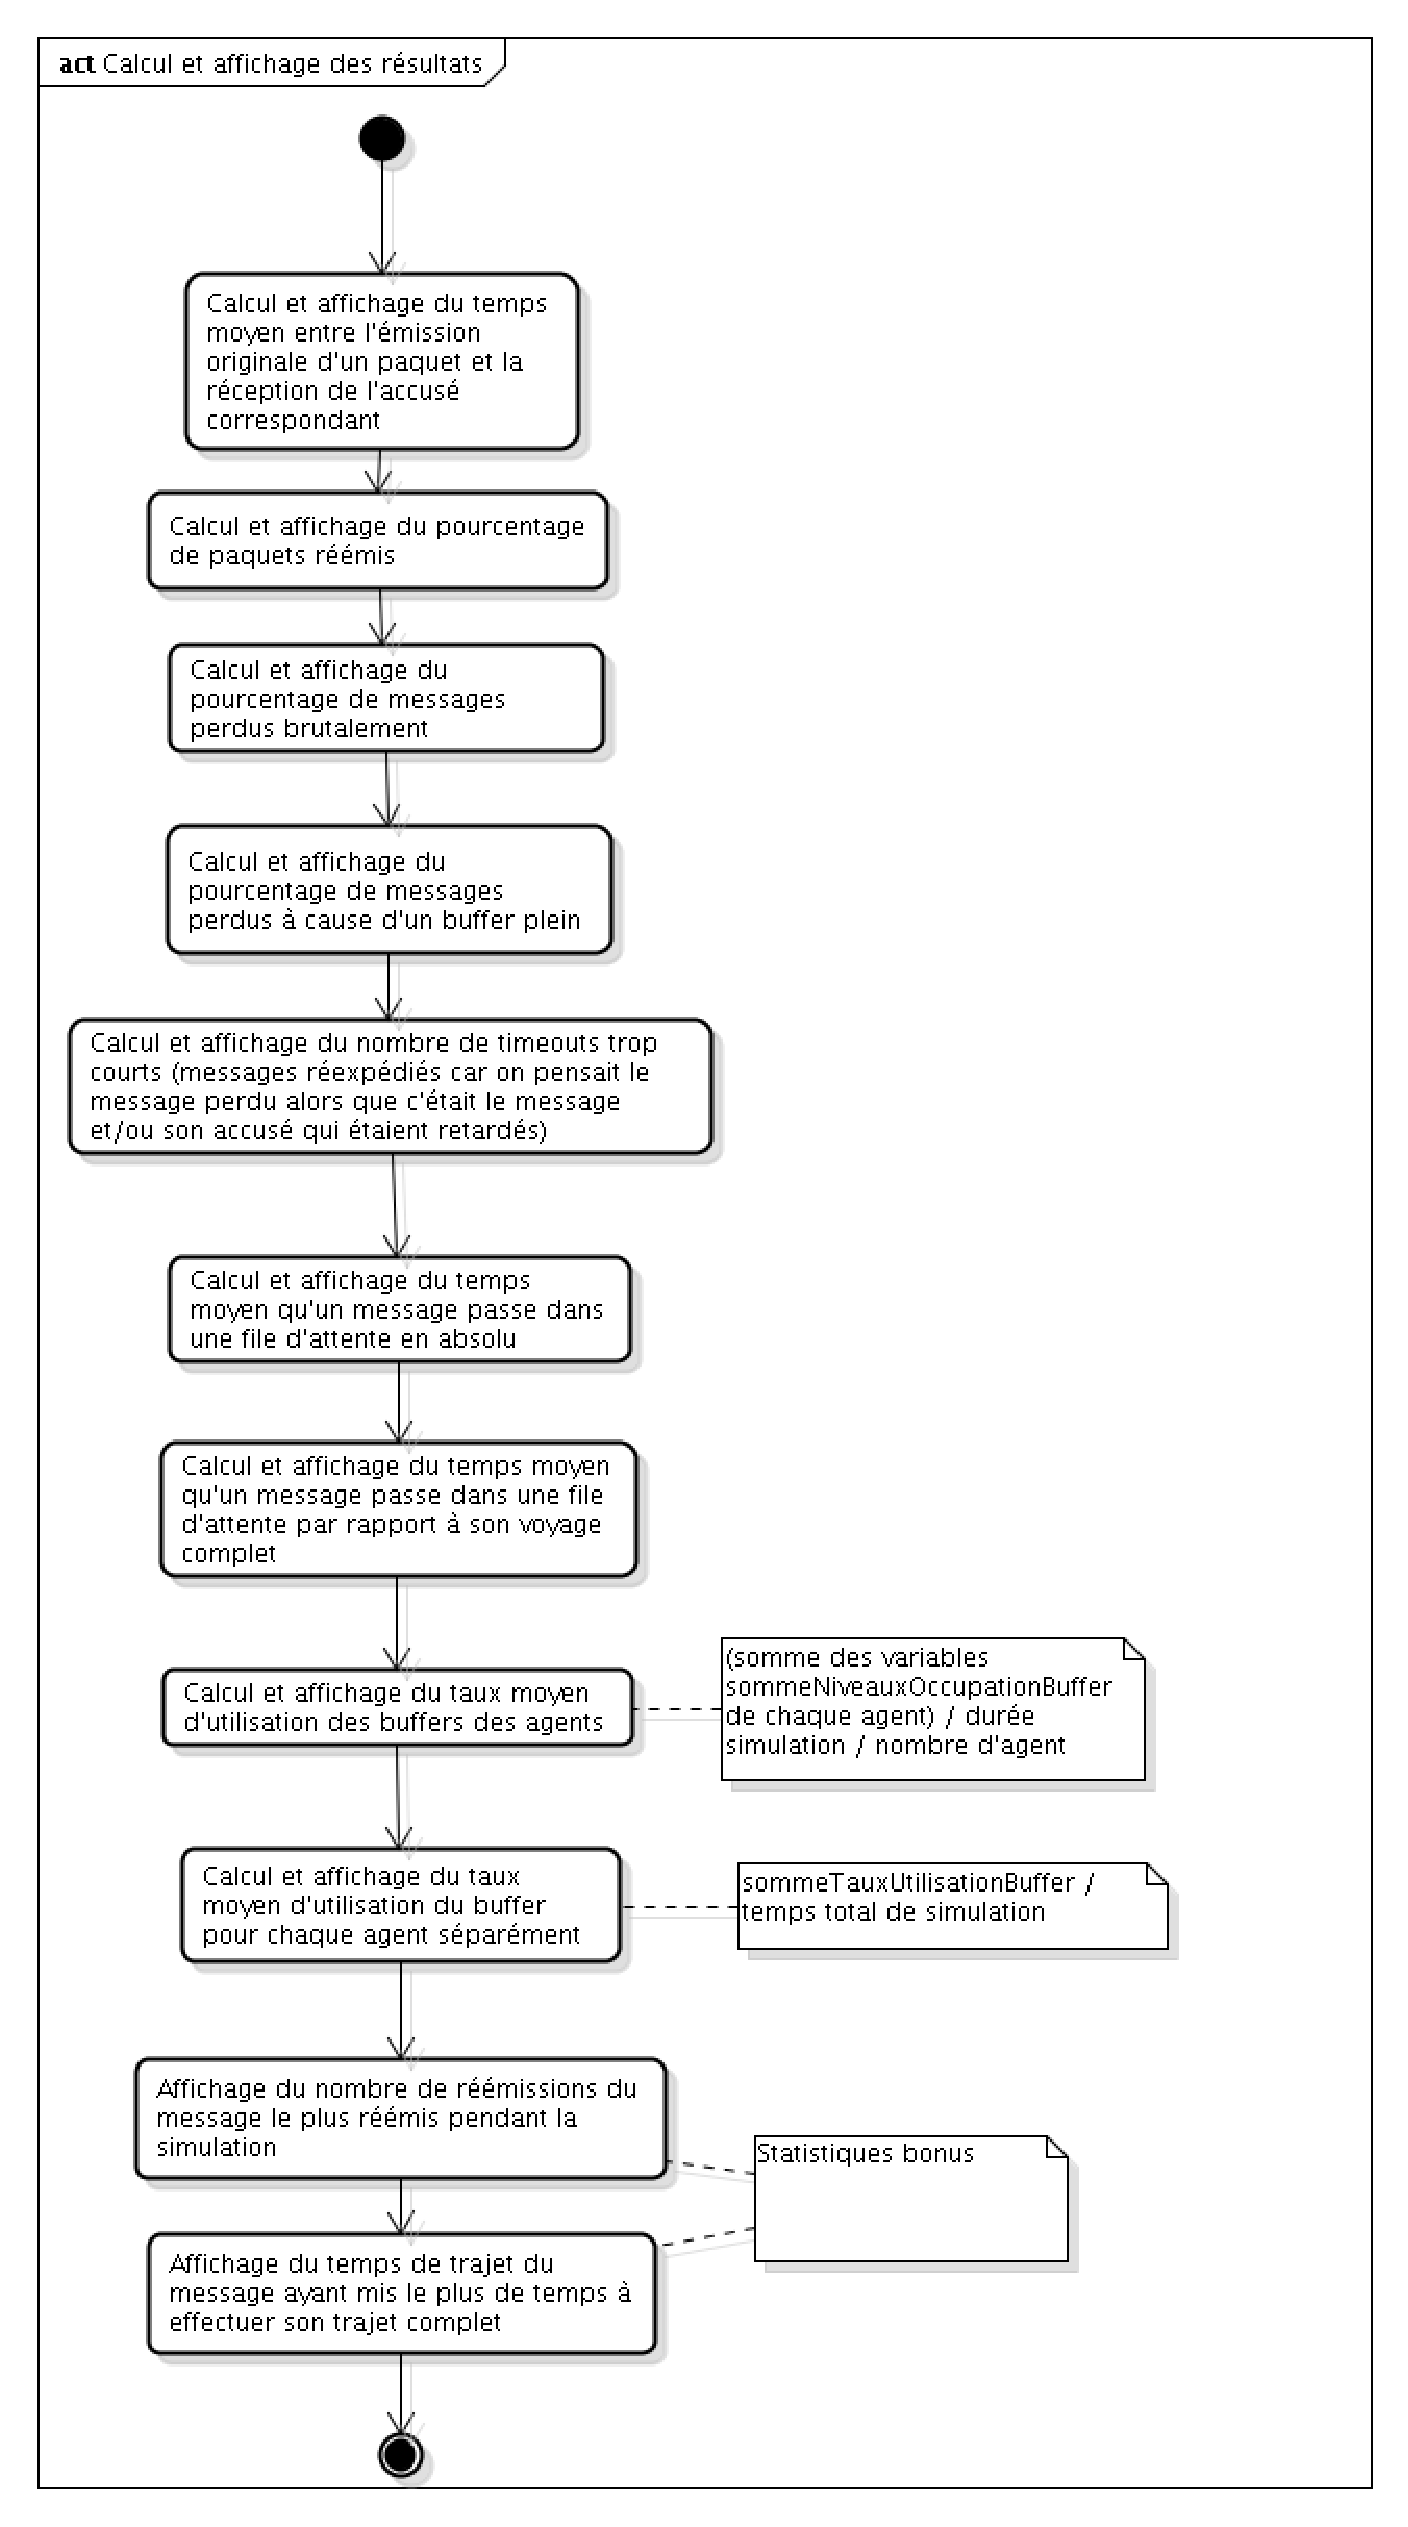
\includegraphics[scale=0.55]{CalculAffichageResultats}
  \caption{Calcul et affichage des résultats}
  \label{fig:calcul-affichage-resultats}
\end{figure}








\section{Résultats}



\subsection{Situation problématique 1}
\subsubsection{Paramètres problématiques}
TODO

\subsubsection{Explications}
TODO

\subsubsection{Résolution du problème}
TODO




\subsection{Situation problématique 2}
\subsubsection{Paramètres problématiques}
TODO

\subsubsection{Explications}
TODO

\subsubsection{Résolution du problème}
TODO





\subsection{Amélioration apportée par le DV}
TODO







%\pagebreak
\clearpage

%\backmatter % pour ne pas numéroter à la fin
\appendix

\section{Le programme et son utilisation}
L'exécutable du projet est disponible dans le dossier \textbf{target/dist}. Pour l'exécuter, il suffit d'ouvrir un prompt et de lancer: \textbf{java -jar simulation.jar}.

\subsection{Configuration et aide}
Pour afficher la liste des paramètres pouvant être donnés au programme, il suffit d'ouvrir un prompt et de lancer: \textbf{java -jar simulation.jar --aide}


\begin{figure}[h!t]
  \centering
    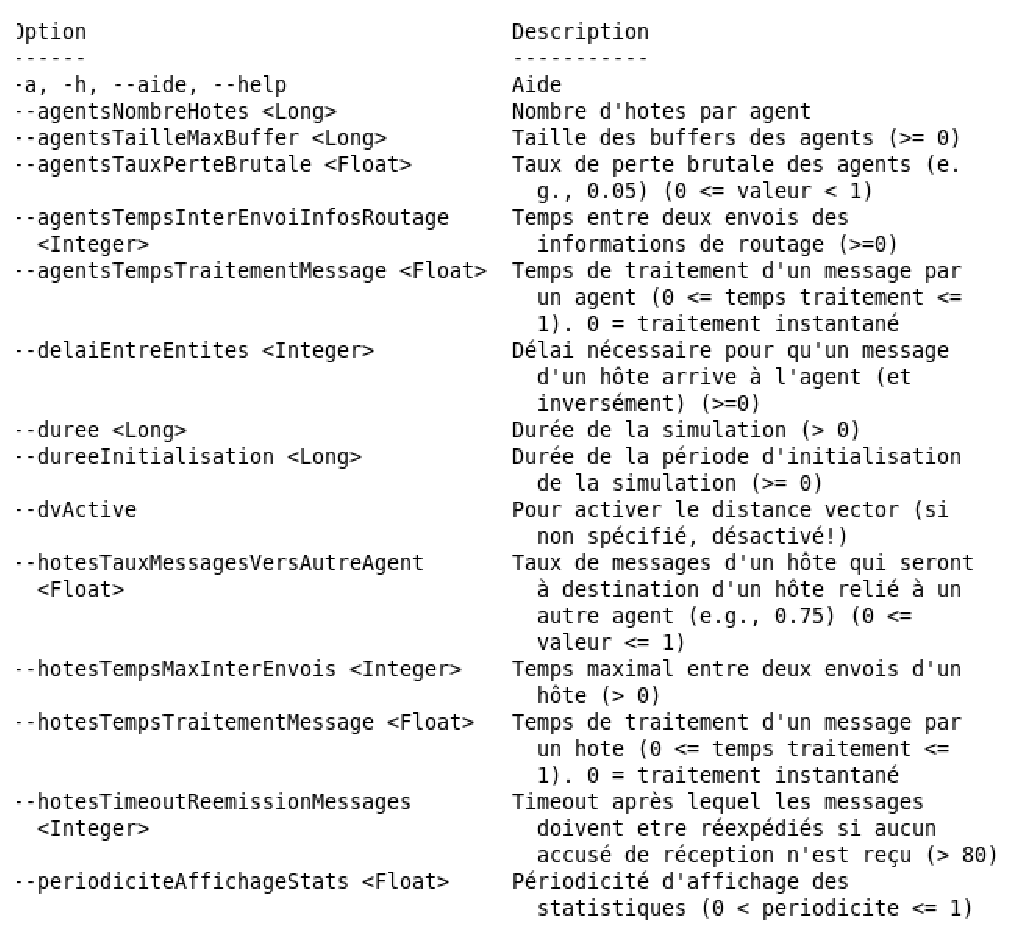
\includegraphics[scale=0.65]{options.eps}
  \caption{Options disponibles}
  \label{fig:options}
\end{figure}

Ensuite pour spécifier les options, on peut par exemple faire: \textbf{java -jar simulation.jar --agentNombreHotes 1000 --duree 5000}.

\subsection{Organisation du code source}
\begin{itemize}
 \item Les sources se trouvent dans le dossier \textbf{src/main/java}
 \item Les fichiers de configuration par défaut se trouvent dans le dossier \textbf{src/main/resources/configuration}
\end{itemize}

Le point d'entrée du programme est la classe \textit{Main} qui se trouve dans \textbf{src/main/java/be/simulation}.

\subsection{Exécution de la simulation}
Lancer le programme exécute directement la simulation. Si aucune option n'est spécifiée en argument au programme, les valeurs par défaut sont utilisées. Les résultats sont affichés à l'écran et sauvegardés dans un fichier de log.

\subsection{Compilation}
La compilation du code requiert l'utilisation de Maven \footnote{\url{http://maven.apache.org/}}, un outil de build très simple d'utilisation. En étant dans le dossier du projet (au niveau où se trouve le fichier \textbf{pom.xml}), il suffit d'exécuter la commande suivante: \textbf{mvn package}. Une fois terminé, le fichier jar exécutable est disponible dans le dossier \textbf{target/dist}.

Maven est très simple à installer sur la plupart des distributions Linux (e.g., Ubuntu, ...). Sous Windows, il suffit de le télécharger et d'ajouter le dossier bin au path.



\subsection{UML}
Un diagramme de classes montrant les classes principales du projet existe mais n'a pas été inclus dans le rapport car il est trop grand. Il est disponible dans le dossier \textbf{UML} qui accompagne le rapport (le fichier: \textbf{CD Entites.png}).
\appendix


\end{document}
